%% Manuscript for Data Science and Engineering (Springer Nature).
%% Build with the official Springer Nature LaTeX template (sn-jnl.cls + sn-mathphys-num.bst),
%% e.g. on Overleaf: "Springer Nature LaTeX Template" -> replace its .tex with this file,
%% upload references.bib and the figures/ folder.
\documentclass[pdflatex,sn-mathphys-num]{sn-jnl}

\usepackage{graphicx}
\usepackage{multirow}
\usepackage{amsmath,amssymb,amsfonts}
\usepackage{booktabs}
\usepackage{xcolor}
\usepackage{url}

\newcommand{\Rtrue}{R_{\mathrm{true}}}
\newcommand{\Rest}{R_{\mathrm{est}}}

\raggedbottom

\begin{document}

\title[Decoupling Trust and Danger in Weather-Degraded Driving Perception]{Decoupling Trust from Danger: Runtime Failure Prediction for Weather-Degraded Monocular Driving Perception}

\author[1]{\fnm{Syed} \sur{Arsalan}}\email{syed.arsalan2023@gmail.com}
\author*[1]{\fnm{Kulandai Josephine Julina} \sur{Joseph}}\email{josephinejulina.jk@vit.ac.in}
\affil[1]{\orgdiv{School of Computer Science and Engineering}, \orgname{Vellore Institute of Technology}, \orgaddress{\city{Chennai}, \state{Tamil Nadu}, \country{India}}}

\abstract{Object detectors used for driving perception degrade at night and in adverse weather such as rain, snow and fog, and they degrade without warning: their confidence scores remain high while their outputs deteriorate. For a detector trained mostly on clear daytime imagery, these conditions are out-of-distribution (OOD) inputs. A single fused risk score does not account for this loss of visibility, so a road that looks empty in dense fog receives a low risk score. This paper presents a perception readout with two decoupled axes per frame. \emph{Trust} is a score that ranks frames by how likely the frozen detector's output on each frame is to be correct; it is estimated at runtime without ground truth by a gradient-boosted introspective model over 30 meta-features (confidence statistics, flip-consistency, distance to clear-day data in a self-supervised feature space, raw-frame image quality and weather-classifier outputs). \emph{Danger} is a normalised hazard score computed from the detections; its underestimation is measured by evaluating the same formula on ground-truth annotations. The trust model is trained only on 3,000 clear-day BDD100K frames and tested on 10,824 frames from 21 held-out strata covering unseen weather, two unseen cameras (ACDC, Cityscapes) and synthetic corruptions. With video-level cluster-bootstrap confidence intervals, the pooled failure-prediction AUROC is 0.739 [0.719, 0.757], against 0.610 [0.592, 0.631] for detection confidence, and the excess area under the risk--coverage curve falls by 34\%. Detected danger underestimates the true danger in every stratum, most at night, and the gap grows monotonically with fog density on identical scenes. Frames with low trust and low apparent danger are underestimated by more than 0.1 in 66\% of cases, against 13.5\% in the other quadrants. The limits of the approach are also reported: the gains are not significant on two of the four cross-camera ACDC conditions, and clear-day probability calibration does not transfer to adverse weather. The full system runs at 20.6 frames per second at 720p on a laptop GPU.}

\keywords{Introspective perception, Failure prediction, Selective prediction, Out-of-distribution data, Adverse weather, Object detection, Autonomous driving}

\maketitle

%% =====================================================================
\section{Introduction}\label{sec:intro}
%% =====================================================================

Detecting objects in a real-world scene becomes harder as the environment imposes more demanding constraints. These constraints range from simple, as under normal lighting, to complex, as under dim lighting. The effectiveness of an object detector therefore depends on the nature of the captured data and on environmental constraints such as adverse weather. Objects are detected with relative ease in a clear daytime scene, whereas rain, snow and fog make the task considerably more difficult. Perception models used in driving can also degrade at night, and they do so without any warning: their confidence scores remain high while their outputs deteriorate.

For a detector trained largely on clear daytime imagery, rain, snow, fog and low light produce out-of-distribution (OOD) data, that is, inputs whose statistics differ from those seen during training~\cite{hendrycks2017baseline,ovadia2019trust,yang2024oodsurvey}. Camera-based detectors lose accuracy substantially on such inputs~\cite{michaelis2019winter,bijelic2020seeing,zhang2023adverse}, and the confidence attached to each box becomes a poor estimate of its probability of being correct, with miscalibration growing under distribution shift~\cite{guo2017calibration,ovadia2019trust}. A downstream planner therefore receives detections that it cannot audit. Introspective perception addresses this problem by learning, from features of the perception process itself, to predict when perception will fail~\cite{daftry2016introspective,rabiee2019ivoa,rabiee2023introspective}, and runtime monitoring of perception networks has become an active area of safety research~\cite{schotschneider2025runtime}. A vehicle that can recognise unreliable perception is able to slow down, request a second sensor or return control to a driver.

Many driving-risk pipelines go a step further and fuse perception confidence and scene hazard into a single number. Such fusion hides the most dangerous failure mode. On an apparently empty road in dense fog, the detector returns no boxes and a fused score reports low risk. The scene in fact combines \emph{low apparent danger} with \emph{low trust}: it appears safe precisely because the detector may be missing the pedestrian in it. Recognising this situation requires the two quantities to be estimated and reported separately.

A two-axis readout of this kind raises three practical challenges:
\begin{enumerate}
\item[(i)] Failure has to be predicted without ground truth and under shifts absent from training. No annotation is available at deployment, and adverse-weather data with box annotations is scarce. A useful introspective model must be trained on plentiful clear-weather data and still rank frames correctly in weather, and on cameras, that it has never encountered. Its evaluation must also separate weather shift from camera shift.
\item[(ii)] Danger estimated from detections is biased, and the bias is rarely measured. A hazard score computed on detected objects inherits every missed detection. Quantifying this bias requires computing the same score on ground truth, which earlier work on risk estimation from monocular video seldom does.
\item[(iii)] Small evaluation sets with correlated frames inflate apparent gains. Adverse-weather benchmarks contain few sequences (ACDC has 6--12 recordings per condition), and consecutive frames are strongly correlated. Per-condition point estimates reported without uncertainty can suggest consistent improvements that the data do not support.
\end{enumerate}

To address these challenges, this work builds and evaluates a confidence-aware, weather-adaptive perception pipeline for monocular driving video (Fig.~\ref{fig:pipeline}). The main contributions are as follows:
\begin{itemize}
\item A decoupled trust--danger readout. Trust is predicted by a lightweight gradient-boosted introspective model over 30 runtime meta-features from five families, trained on clear-day data only. Danger is a normalised hazard score whose underestimation is measured against the same score computed on annotations.
\item A shift-stratified evaluation protocol over 13,824 frames from BDD100K, ACDC, Cityscapes/Foggy Cityscapes and synthetic corruptions. The protocol separates weather shift from camera shift through paired clear and foggy renderings of identical scenes, and every result is reported with video-level cluster-bootstrap confidence intervals and selective-prediction metrics.
\item Empirical findings on what transfers and what does not. Failure \emph{ranking} transfers to unseen weather (pooled AUROC 0.739 vs.\ 0.610 for confidence; E-AURC reduced by 34\%), whereas clear-day \emph{calibration} does not; danger is underestimated in every stratum; and the low-trust, low-danger quadrant isolates the frames in which danger is most underestimated. A controlled comparison of three detector generations under weather, a tested adaptive-enhancement stage and a real-time implementation are also reported.
\end{itemize}

The remainder of the paper is organised as follows. Section~\ref{sec:related} reviews related work, Section~\ref{sec:method} describes the methodology, Section~\ref{sec:exp} presents the experimental protocol and results, and Section~\ref{sec:discussion} discusses limitations. Section~\ref{sec:conclusion} provides concluding remarks.

\begin{figure*}[t]
\centering
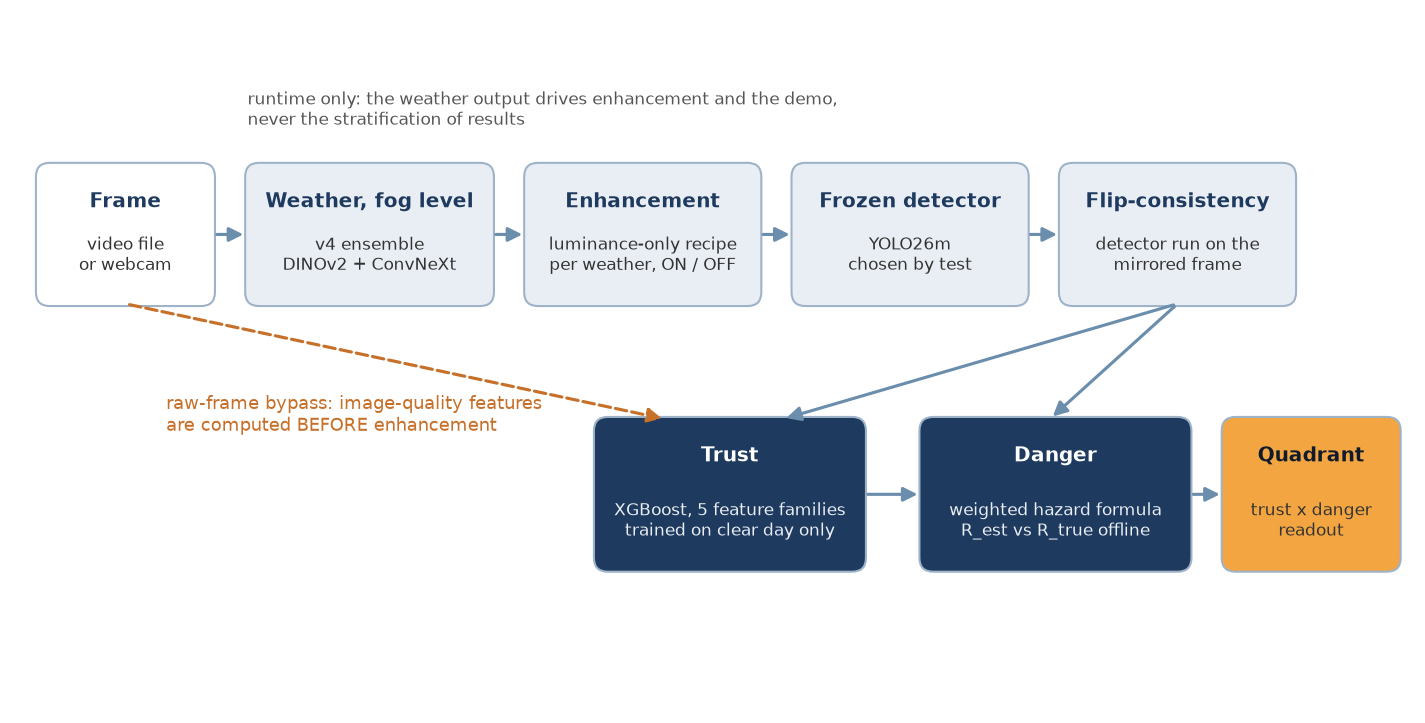
\includegraphics[width=\textwidth]{figures/pipeline.png}
\caption{Overview of the proposed trust--danger pipeline}
\label{fig:pipeline}
\end{figure*}

%% =====================================================================
\section{Related Work}\label{sec:related}
%% =====================================================================

Reliable perception under adverse conditions draws on three lines of research. The first predicts, at runtime, when a perception module is about to fail. The second studies how far a model's own confidence can be trusted, especially on OOD inputs, and how a confidence score should be judged when it is used to accept or reject predictions. The third measures and mitigates the effect of weather on detection itself. This section reviews each line and positions the present work with respect to it.

\textbf{Introspective perception and failure prediction.} Daftry et al.~\cite{daftry2016introspective} introduced introspective perception, in which a model learns from features of the perception process whether a vision system's output will be wrong; the prediction was used to decide when a micro-aerial vehicle should trust its own perception. Rabiee and Biswas applied the idea to stereo obstacle detection~\cite{rabiee2019ivoa} and later generalised it to a framework for introspective perception on mobile robots~\cite{rabiee2023introspective}. Runtime safety monitors for perception networks have recently been surveyed in~\cite{schotschneider2025runtime}. The underlying problem, estimating the performance of a deployed model without access to labels, also arises outside vision: Zoppi et al.~\cite{zoppi2025predicting} predict the performance of supervised and unsupervised tabular classifiers, and FL-GUARD~\cite{lin2024flguard} detects at run time when a federated learning process fails to benefit its clients and triggers recovery. For object detectors, MetaDetect~\cite{schubert2021metadetect} regresses per-box quality from hand-crafted box-level meta-features, and Rahman et al.~\cite{rahman2021online} predict frame-level detection performance online from the detector's internal features. Oksuz et al.~\cite{oksuz2023selfaware} formulate self-aware object detectors that decide at image level whether to accept an input and that calibrate their detection confidences. The present work adopts the frame-level formulation of~\cite{rahman2021online}, but relies only on signals available from a black-box detector, trains on a single condition and evaluates transfer across both weather and camera.

\textbf{Uncertainty, calibration and selective prediction.} Modern networks are overconfident, and temperature scaling corrects this only in distribution~\cite{guo2017calibration}; under dataset shift, the calibration of most uncertainty methods deteriorates~\cite{ovadia2019trust}. Bayesian and ensemble methods~\cite{kendall2017uncertainties,lakshminarayanan2017ensembles} and probabilistic detectors~\cite{feng2022review} improve uncertainty estimates, at the cost of retraining or multiple forward passes of the detector. Calibration of detector confidence has also been extended to box geometry~\cite{kuppers2020multivariate}. The maximum softmax probability is the standard baseline for detecting misclassified and OOD inputs~\cite{hendrycks2017baseline}; its detection analogue, mean box confidence, serves as the baseline in this study. Selective prediction~\cite{geifman2017selective} evaluates a confidence score by the risk incurred when only the most confident fraction of inputs is accepted, summarised by the area under the risk--coverage curve (AURC) and its excess over the optimum (E-AURC)~\cite{geifman2019biasreduced}. Jaeger et al.~\cite{jaeger2023failure} argue that failure detection should be judged with such risk--coverage metrics, since detecting OOD inputs and detecting wrong predictions are not the same task. Feature-space nearest-neighbour distances are effective OOD scores~\cite{sun2022knn,yang2024oodsurvey} and form one of the feature families used here.

\textbf{Robustness of detection to weather.} Benchmarks with synthetic corruptions~\cite{hendrycks2019benchmarking,michaelis2019winter} show large and graded degradation of detectors. Real adverse-weather data is provided by BDD100K~\cite{yu2020bdd100k}, ACDC~\cite{sakaridis2021acdc}, Foggy Cityscapes~\cite{sakaridis2018foggy} and DAWN~\cite{kenk2020dawn}; multimodal fusion with lidar and radar~\cite{bijelic2020seeing} is an alternative where those sensors are available, and the sensing side of the problem is reviewed in~\cite{zhang2023adverse}. Several works improve the detector itself for adverse weather, through domain adaptation to foggy scenes~\cite{li2023foggyda} or by training YOLO-family detectors on merged adverse-weather data~\cite{kumar2023yolov8adverse} or with fog-specific architectural changes~\cite{kuang2026fogyolo}. These approaches retrain the detector; the present work keeps it frozen and estimates instead when its output can be trusted. Image restoration as a pre-processing step does not necessarily help recognition~\cite{pei2018haze}, which motivated jointly learned enhancement such as IA-YOLO~\cite{liu2022iayolo}. Here, classical enhancement~\cite{he2011darkchannel,zuiderveld1994clahe} is treated as a hypothesis to be tested, with an explicit check that it does not inflate confidence.

%% =====================================================================
\section{Methodology}\label{sec:method}
%% =====================================================================

\subsection{Problem Formulation}

Let $x_t$ be the frame at time $t$ and $D(x_t) = \{(b_i, c_i, s_i)\}$ the boxes, classes and confidences returned by a frozen detector $D$. Annotations $G_t$ are available only offline. Detections are matched greedily and one-to-one to annotations of the same class at an intersection-over-union of 0.5, and boxes shorter than 12 pixels are ignored. A frame is labelled a \emph{failure} when its detection F1 score is below 0.5 or at least one annotated pedestrian is missed:
\begin{equation}
y_t = \mathbb{1}\!\left[\,\mathrm{F1}_t < 0.5 \;\lor\; M_t > 0\,\right],
\label{eq:failure}
\end{equation}
where $M_t$ is the number of missed pedestrians. The pedestrian clause makes the label safety-relevant: a frame in which every car is found but a person is missed counts as a failure.

Two quantities are sought that can be computed at runtime without $G_t$. The first is a trust score,
\begin{equation}
T(x_t) = 1 - \hat{P}\!\left(y_t = 1 \mid \phi(x_t)\right) \in [0,1],
\label{eq:trust}
\end{equation}
where $\phi(x_t)$ is a meta-feature vector and $\hat{P}$ is the failure probability estimated by the introspective model. Although $T$ is derived from a probability estimate, it is used as a failure-ranking score: Sect.~\ref{sec:calib} shows that the estimated probabilities are not calibrated under shift, so a probabilistic reading of $T$ is valid only for conditions in which calibration has been verified. The second is a danger score $\Rest(x_t) = R(D(x_t), w_t) \in [0,1]$, where $w_t$ denotes the weather condition and $R$ is defined in Sect.~\ref{sec:danger}. Offline, the same function evaluated on the annotations gives $\Rtrue = R(G_t, w_t)$, and the danger gap is
\begin{equation}
\Delta_t = \Rtrue(x_t) - \Rest(x_t).
\label{eq:gap}
\end{equation}
A positive $\Delta_t$ means that perception underestimates the danger of the scene.

\subsection{Weather Classifier}

A classifier with a shared backbone and three heads predicts the condition (clear, fog, night, rain, snow), a fog level and a rain level. The fog levels (none, light, medium, dense) are tied to the Foggy Cityscapes attenuation coefficients $\beta \in \{0.005, 0.01, 0.02\}$, which correspond to a visibility of roughly 600, 300 and 150\,m~\cite{sakaridis2018foggy}. The final model ensembles a DINOv2 ViT-S/14~\cite{oquab2024dinov2} with its last two blocks fine-tuned and a fully fine-tuned ConvNeXt-Tiny~\cite{liu2022convnext}, with mirror test-time averaging. It is trained on 54,822 BDD100K images, ACDC, clean, foggy and rainy Cityscapes, and on fog rendered onto clear frames of every camera. The rendering uses monocular depth~\cite{yang2024depthv2} and the atmospheric scattering model,
\begin{equation}
I(x) = J(x)\,e^{-\beta d(x)} + A\left(1 - e^{-\beta d(x)}\right),
\label{eq:fog}
\end{equation}
where $J$ is the clear image, $d$ the estimated depth, $A$ the atmospheric light and $\beta$ the attenuation coefficient, calibrated against the three Foggy Cityscapes levels. Augmentation is geometric and camera-agnostic only; brightness and contrast are never perturbed, since they carry the fog and night cues.

During development, the classifier exhibited a \emph{camera shortcut}. A model trained without clean Cityscapes frames scored 100\% on foggy Cityscapes but labelled 59 of 60 \emph{clear} Cityscapes frames as fog: it had learned to recognise the camera rather than the weather. Including clean frames from every camera removed the shortcut, and leave-one-camera-out accuracy is therefore reported as the realistic generalisation figure. The weather classifier is used only at runtime, to select the enhancement recipe and as a trust feature. All evaluation strata are defined by the datasets' own weather tags, so classification errors cannot alter the experimental conditions.

\subsection{Trust Features and Model}\label{sec:trust}

The meta-feature vector $\phi(x_t) \in \mathbb{R}^{30}$ comprises five families:
\begin{enumerate}
\item Confidence statistics (11 features): number of detections and of persons; mean, maximum, minimum and standard deviation of confidence; fraction of boxes below 0.5 and above 0.8; mean box area; class entropy; and number of small boxes.
\item Flip-consistency (4): the detector is re-run on the horizontally mirrored frame and its boxes are mapped back. The features are the Dice overlap of the two box sets, the confidence agreement of matched pairs, the count difference and a person-only Dice overlap. This family stands in for temporal persistence, which is unavailable on single-frame benchmarks.
\item Feature-space distance (3): with $z(x)$ the DINOv2 embedding of a frame and $\mathcal{N}_k(x)$ its $k=5$ nearest clear-day training embeddings, the mean distance is
\begin{equation}
d_{\mathrm{kNN}}(x) = \frac{1}{k}\sum_{j \in \mathcal{N}_k(x)} \left(1 - \frac{z(x)^\top z_j}{\lVert z(x)\rVert\,\lVert z_j\rVert}\right),
\label{eq:knn}
\end{equation}
complemented by the minimum distance and the distance to the mean training embedding~\cite{sun2022knn}.
\item Raw-frame image quality (6): Laplacian variance, RMS contrast, mean brightness, dark-channel haze estimate~\cite{he2011darkchannel}, saturation and edge density. These are computed on the frame \emph{before} enhancement, so that enhancement cannot mask the degradation they measure.
\item Weather (6): the classifier's five condition probabilities and its fog level.
\end{enumerate}

An XGBoost classifier~\cite{chen2016xgboost} with 400 trees, depth 4, learning rate 0.05, row and column subsampling of 0.8 and class weighting is fitted to predict $y_t$ from $\phi(x_t)$ on clear-day frames only, and trust follows from Eq.~(\ref{eq:trust}). Training on a single condition is a deliberate choice. It makes every adverse stratum a genuine test of transfer, and it mirrors the practical situation in which annotated clear-weather data is far more plentiful than annotated adverse-weather data.

\subsection{Danger Score}\label{sec:danger}

Each object $j$ with class $c_j$ and box $b_j$ contributes $w_{c_j} \cdot \rho(b_j)$. The class weight $w_c$ is 1.0 for persons, 0.9 for bicycles and motorcycles, 0.6 for trucks and buses, 0.5 for cars and 0.1 for traffic lights. The relevance $\rho(b) \in [0,1]$ increases with box size, with lowness in the image (proximity under a flat-ground assumption) and with horizontal centrality (proximity to the ego path). The object term saturates and is combined with a weather-severity term $\sigma(w)$:
\begin{equation}
R = 0.7\left(1 - \exp\Big(-3\sum_j w_{c_j}\,\rho(b_j)\Big)\right) + 0.3\,\sigma(w),
\label{eq:danger}
\end{equation}
with $\sigma = 0$ for clear weather, 0.4 for rain, 0.5 for night and snow, and 0.5--0.9 for fog depending on its level. The same weather term enters both $\Rest$ and $\Rtrue$, so the gap in Eq.~(\ref{eq:gap}) isolates the distortion introduced by detection. Since the weights are set by hand, their influence is tested by perturbing each one by $\pm 50\%$ (Sect.~\ref{sec:res_danger}).

\subsection{Weather-Adaptive Enhancement}

Enhancement operates on luminance only, and clear frames are left untouched. Light fog receives contrast-limited adaptive histogram equalisation (CLAHE)~\cite{zuiderveld1994clahe}. Medium and dense fog receive dark-channel dehazing~\cite{he2011darkchannel} with guided-filter refinement, a transmission floor and a sky guard, followed by CLAHE and, for dense fog, a bilateral denoising step. Night frames receive adaptive gamma correction towards a target mean luminance of 0.45, CLAHE and a bilateral filter; rain frames receive CLAHE; and over-bright snow frames receive a gamma above one and CLAHE. Every experiment is run with enhancement both on and off, and the mean confidence of true positives is tracked to detect enhancement that inflates confidence without improving correctness.

\subsection{Decoupled Readout}

At runtime each frame is placed in the trust--danger plane. Frames with $T < 0.5$ and $\Rest < 0.4$ are flagged as \emph{low trust, low apparent danger}, the case that a fused score would report as safe.

%% =====================================================================
\section{Experiments}\label{sec:exp}
%% =====================================================================

\subsection{Datasets and Evaluation Strata}

All data used are public. BDD100K~\cite{yu2020bdd100k} provides 2D boxes and per-image weather and time-of-day tags; ACDC~\cite{sakaridis2021acdc} provides detection annotations for real adverse conditions; Cityscapes~\cite{cordts2016cityscapes}, with boxes derived from its gtFine instance masks, is paired with Foggy Cityscapes-DBF~\cite{sakaridis2018foggy}; and DAWN~\cite{kenk2020dawn} serves as an external test for weather classification. Classes are mapped to a seven-class vocabulary: person (including riders), car, truck, bus, bicycle, motorcycle and traffic light.

The evaluation strata, drawn with a fixed seed, comprise 12,024 real frames (3,000 used to train the trust model and 9,024 held out) and 1,800 synthetic corruptions, so that 10,824 held-out frames form 21 test strata (Table~\ref{tab:strata}). They separate three kinds of shift relative to the trust training data: weather only (BDD100K validation night, rain and snow), camera and weather (ACDC), and camera with controlled weather (the same 800 Cityscapes scenes, clear and at three fog densities, with identical annotations). Synthetic fog, frost and motion blur at severities 1, 3 and 5~\cite{hendrycks2019benchmarking} are applied to 200 held-out clear BDD100K frames, so that severity is the only variable. The synthetic fog of this benchmark is a texture overlay without depth and is therefore less physically realistic than the Foggy Cityscapes renderings.

\begin{table}[t]
\caption{Evaluation strata. ``Seq.'' is the number of distinct videos or recordings, which is the resampling unit of the bootstrap. Real frames: 3,000 for training and 9,024 held out (12,024); with the 1,800 synthetic frames, 10,824 held-out frames form 21 test strata}
\label{tab:strata}
\footnotesize
\begin{tabular}{@{}llrr@{}}
\toprule
Stratum & Shift vs.\ training & Frames & Seq. \\
\midrule
BDD train clear (trust training) & none & 3,000 & -- \\
BDD val clear & none (held out) & 1,500 & 1,274 \\
BDD val night & weather & 1,500 & 1,159 \\
BDD val rain & weather & 396 & 291 \\
BDD val snow & weather & 422 & 306 \\
ACDC fog / night / rain / snow & camera + weather & 500 / 506 / 500 / 500 & 11 / 6 / 11 / 12 \\
Cityscapes clear + 3 fog levels & camera (+ fog) & 800 $\times$ 4 & 493 \\
Synthetic fog, frost, blur (sev.\ 1, 3, 5) & corruption & 200 each & 166 \\
\bottomrule
\end{tabular}
\end{table}

\subsection{Metrics and Statistical Protocol}\label{sec:metrics}

Detection is evaluated by VOC-style AP50, precision and pedestrian recall at an operating confidence of 0.25. Trust is evaluated as a ranking of frames by the AUROC of predicting failure, which equals the probability that a randomly chosen failed frame receives lower trust than a randomly chosen correct frame (0.5 is chance, 1 is perfect).

Trust is also evaluated as a selective predictor. Let the $n$ frames be sorted by decreasing trust and let $y_{(i)}$ denote the failure label of the $i$-th frame. The risk at coverage $m/n$ and the area under the risk--coverage curve are
\begin{equation}
r\!\left(\tfrac{m}{n}\right) = \frac{1}{m}\sum_{i=1}^{m} y_{(i)}, \qquad
\mathrm{AURC} = \frac{1}{n}\sum_{m=1}^{n} r\!\left(\tfrac{m}{n}\right).
\label{eq:aurc}
\end{equation}
Because AURC also depends on the overall failure rate $\bar{r}$, the excess over the best attainable ranking is reported as well~\cite{geifman2019biasreduced}:
\begin{equation}
\mathrm{E\text{-}AURC} = \mathrm{AURC} - \left[\bar{r} + (1-\bar{r})\ln(1-\bar{r})\right].
\label{eq:eaurc}
\end{equation}
The residual failure rate at fixed coverage, i.e.\ when acting only on the most-trusted fraction of frames, is reported alongside. Calibration of the predicted failure probability $p_t = 1 - T(x_t)$ is measured by the Brier score and by the expected calibration error over $B=10$ equal-width bins $\mathcal{B}_b$,
\begin{equation}
\mathrm{ECE} = \sum_{b=1}^{B} \frac{|\mathcal{B}_b|}{n}\,\Big|\,\bar{p}_b - \bar{y}_b\,\Big|,
\label{eq:ece}
\end{equation}
where $\bar{p}_b$ and $\bar{y}_b$ are the mean predicted probability and the observed failure rate in bin $b$. Danger is evaluated by the mean gap $\Delta$, the fraction of frames underestimated by more than 0.1, and the Spearman correlation between $\Rest$ and $\Rtrue$.

Frames from the same video are correlated, and ACDC contains only 6--12 recordings per condition. All confidence intervals are therefore 95\% percentile intervals from a \emph{cluster} bootstrap~\cite{efron1993bootstrap} that resamples whole videos or recordings ($B = 2{,}000$ resamples). For the difference between trust and the confidence baseline, a paired bootstrap on the same resamples is used, and an improvement is regarded as significant when the interval of the difference excludes zero.

\subsection{Implementation Details}

The experiments use Python 3.12, PyTorch 2.11 with CUDA 12.8, Ultralytics 8.4~\cite{ultralytics}, XGBoost~\cite{chen2016xgboost} and scikit-learn on a laptop with an NVIDIA RTX 5060 GPU (8\,GB). Detections are stored down to a confidence of 0.05 so that thresholds can be re-applied without re-running the detector. The only trained components are the weather classifier and the trust model; the detector and the DINOv2 feature extractor used for trust are frozen.

\subsection{Detector Selection Under Weather}

Confidence behaves differently across detectors, so the whole pipeline is built on a single detector, chosen by a rule fixed before the run: the best adverse-weather pedestrian recall among models whose precision lies within five points of the best, with the smallest clear-to-adverse drop as the tie-breaker. Three COCO-pretrained generations of the YOLO family~\cite{ultralytics,terven2023yolo} were compared on identical frames (Table~\ref{tab:detectors}). YOLO26m satisfies the rule and also degrades least from clear to adverse conditions, and it is used throughout.

\begin{table}[t]
\caption{Three detector generations on identical frames, enhancement off. Adverse = night, rain, snow and fog strata of all cameras}
\label{tab:detectors}
\begin{tabular}{@{}lccc@{}}
\toprule
& YOLO26m & YOLO11m & YOLOv8m \\
\midrule
Pedestrian recall, adverse & \textbf{0.443} & 0.409 & 0.413 \\
Precision, adverse & 0.688 & \textbf{0.714} & 0.681 \\
mAP50, adverse & \textbf{0.409} & 0.385 & 0.379 \\
Pedestrian recall, clear & \textbf{0.477} & 0.446 & 0.459 \\
Drop clear $\rightarrow$ adverse & \textbf{0.034} & 0.037 & 0.046 \\
\bottomrule
\end{tabular}
\end{table}

The per-stratum behaviour of YOLO26m shows how strongly each condition affects detection (Table~\ref{tab:detection}). Night is the hardest real condition: ACDC night reaches an mAP50 of only 0.244, and a pedestrian is missed in 55\% of its frames. On the paired Cityscapes scenes, where the annotations are identical across rows, mAP50 falls from 0.457 (clear) to 0.387 (dense fog) and pedestrian recall from 0.461 to 0.398, a weather effect of about seven points with no change of camera. Under synthetic corruption at severity 5, mAP50 falls from 0.475 to 0.447 (fog), 0.275 (frost) and 0.144 (motion blur).

\begin{table}[t]
\caption{YOLO26m detection per stratum, enhancement off. ``Missed ped.'' is the fraction of frames in which at least one annotated pedestrian is missed; ``Fail'' is the failure rate used as the trust label. The high miss rate on Cityscapes reflects its dense annotation of small and occluded people}
\label{tab:detection}
\begin{tabular}{@{}lccccc@{}}
\toprule
Stratum & mAP50 & Ped.\ recall & Precision & Missed ped. & Fail \\
\midrule
BDD val clear & 0.475 & 0.493 & 0.808 & 0.286 & 0.368 \\
BDD val night & 0.335 & 0.352 & 0.707 & 0.182 & 0.571 \\
BDD val rain & 0.493 & 0.468 & 0.803 & 0.283 & 0.359 \\
BDD val snow & 0.441 & 0.542 & 0.800 & 0.296 & 0.370 \\
ACDC fog & 0.545 & 0.559 & 0.613 & 0.148 & 0.316 \\
ACDC night & 0.244 & 0.322 & 0.553 & 0.547 & 0.721 \\
ACDC rain & 0.355 & 0.349 & 0.572 & 0.278 & 0.498 \\
ACDC snow & 0.428 & 0.553 & 0.592 & 0.418 & 0.564 \\
Cityscapes clear & 0.457 & 0.461 & 0.741 & 0.671 & 0.700 \\
Cityscapes fog light & 0.440 & 0.450 & 0.741 & 0.676 & 0.703 \\
Cityscapes fog medium & 0.425 & 0.433 & 0.744 & 0.682 & 0.718 \\
Cityscapes fog dense & 0.387 & 0.398 & 0.752 & 0.705 & 0.741 \\
\bottomrule
\end{tabular}
\end{table}

\subsection{Failure Prediction}\label{sec:res_trust}

The central question for the trust model is whether it orders frames correctly: frames on which the detector fails should receive lower trust than frames on which it succeeds, including under weather and cameras absent from training. This ordering is measured by the AUROC defined in Sect.~\ref{sec:metrics}, and each value is compared with the same measure computed from mean detection confidence. The results, with cluster-bootstrap intervals, are listed in Table~\ref{tab:trust} and shown in Fig.~\ref{fig:forest}. Pooled over all 21 held-out strata (10,824 frames, 3,437 sequences), trust reaches 0.739 [0.719, 0.757], against 0.610 [0.592, 0.631] for mean confidence, a paired improvement of +0.129 [+0.102, +0.155]. Over the 12 real adverse strata the improvement is +0.141 [+0.108, +0.171].

The trust point estimate exceeds the baseline in all 21 strata, but the interval of the difference excludes zero in 13 of them. The gain is significant on every stratum from the training camera (BDD100K, +0.08 to +0.16), on all four Cityscapes rows (+0.06 to +0.08), and on ACDC night (+0.09) and snow (+0.05). It is not significant on ACDC fog and rain, whose intervals are wide because each contains only 11 recordings, nor on most of the 200-frame synthetic strata. On synthetic fog in particular, mean confidence is already a strong signal (0.71--0.75), which leaves little room for improvement.

Transfer weakens with the kind of shift. Under weather shift alone (BDD100K), AUROC stays between 0.73 and 0.76, close to the in-distribution value of 0.761. Under a new camera with controlled fog (Cityscapes) it lies between 0.73 and 0.74 and does not decline as the fog thickens. Under a new camera with real weather (ACDC) it falls to 0.64--0.66. The Cityscapes rows indicate that a change of camera alone does not explain the drop on ACDC; the combination of a new camera and real weather does.

\begin{table}[t]
\caption{Failure prediction: AUROC with 95\% cluster-bootstrap intervals, paired difference (trust $-$ confidence) and residual failure rate when acting on the most-trusted 50\% of frames. $^\ast$: interval of the difference excludes 0}
\label{tab:trust}
\footnotesize
\setlength{\tabcolsep}{4pt}
\begin{tabular}{@{}lccccc@{}}
\toprule
Stratum & Fail rate & AUROC trust & AUROC conf. & $\Delta$AUROC & Fail@50\% \\
\midrule
BDD val clear & 0.368 & 0.761 [.735, .786] & 0.654 & +0.107$^\ast$ & 0.197 \\
BDD val night & 0.571 & 0.730 [.706, .753] & 0.651 & +0.078$^\ast$ & 0.409 \\
BDD val rain & 0.359 & 0.750 [.694, .801] & 0.592 & +0.158$^\ast$ & 0.207 \\
BDD val snow & 0.370 & 0.729 [.677, .777] & 0.619 & +0.110$^\ast$ & 0.227 \\
ACDC fog & 0.316 & 0.644 [.607, .689] & 0.603 & +0.041 & 0.228 \\
ACDC night & 0.721 & 0.637 [.550, .704] & 0.544 & +0.092$^\ast$ & 0.652 \\
ACDC rain & 0.498 & 0.663 [.607, .723] & 0.612 & +0.050 & 0.380 \\
ACDC snow & 0.564 & 0.656 [.603, .705] & 0.605 & +0.051$^\ast$ & 0.444 \\
Cityscapes clear & 0.700 & 0.731 [.687, .765] & 0.648 & +0.083$^\ast$ & 0.545 \\
Cityscapes fog light & 0.703 & 0.733 [.686, .773] & 0.656 & +0.078$^\ast$ & 0.563 \\
Cityscapes fog medium & 0.718 & 0.733 [.686, .772] & 0.670 & +0.063$^\ast$ & 0.585 \\
Cityscapes fog dense & 0.741 & 0.744 [.700, .782] & 0.676 & +0.068$^\ast$ & 0.598 \\
Synthetic fog 1 & 0.425 & 0.774 [.709, .833] & 0.750 & +0.024 & 0.250 \\
Synthetic fog 3 & 0.440 & 0.765 [.699, .827] & 0.745 & +0.021 & 0.280 \\
Synthetic fog 5 & 0.465 & 0.761 [.691, .824] & 0.711 & +0.050 & 0.260 \\
Synthetic frost 1 & 0.450 & 0.807 [.745, .865] & 0.662 & +0.145$^\ast$ & 0.250 \\
Synthetic frost 3 & 0.600 & 0.742 [.674, .804] & 0.680 & +0.062 & 0.420 \\
Synthetic frost 5 & 0.600 & 0.732 [.663, .797] & 0.637 & +0.094$^\ast$ & 0.420 \\
Synthetic blur 1 & 0.460 & 0.728 [.652, .794] & 0.682 & +0.046 & 0.310 \\
Synthetic blur 3 & 0.590 & 0.680 [.601, .754] & 0.603 & +0.076 & 0.460 \\
Synthetic blur 5 & 0.815 & 0.684 [.548, .798] & 0.569 & +0.115$^\ast$ & 0.730 \\
\midrule
Pooled, 21 held-out & 0.556 & 0.739 [.719, .757] & 0.610 & +0.129$^\ast$ & 0.382 \\
Pooled, 12 real adverse & 0.586 & 0.722 [.702, .742] & 0.581 & +0.141$^\ast$ & 0.425 \\
\bottomrule
\end{tabular}
\end{table}

\begin{figure}[t]
\centering
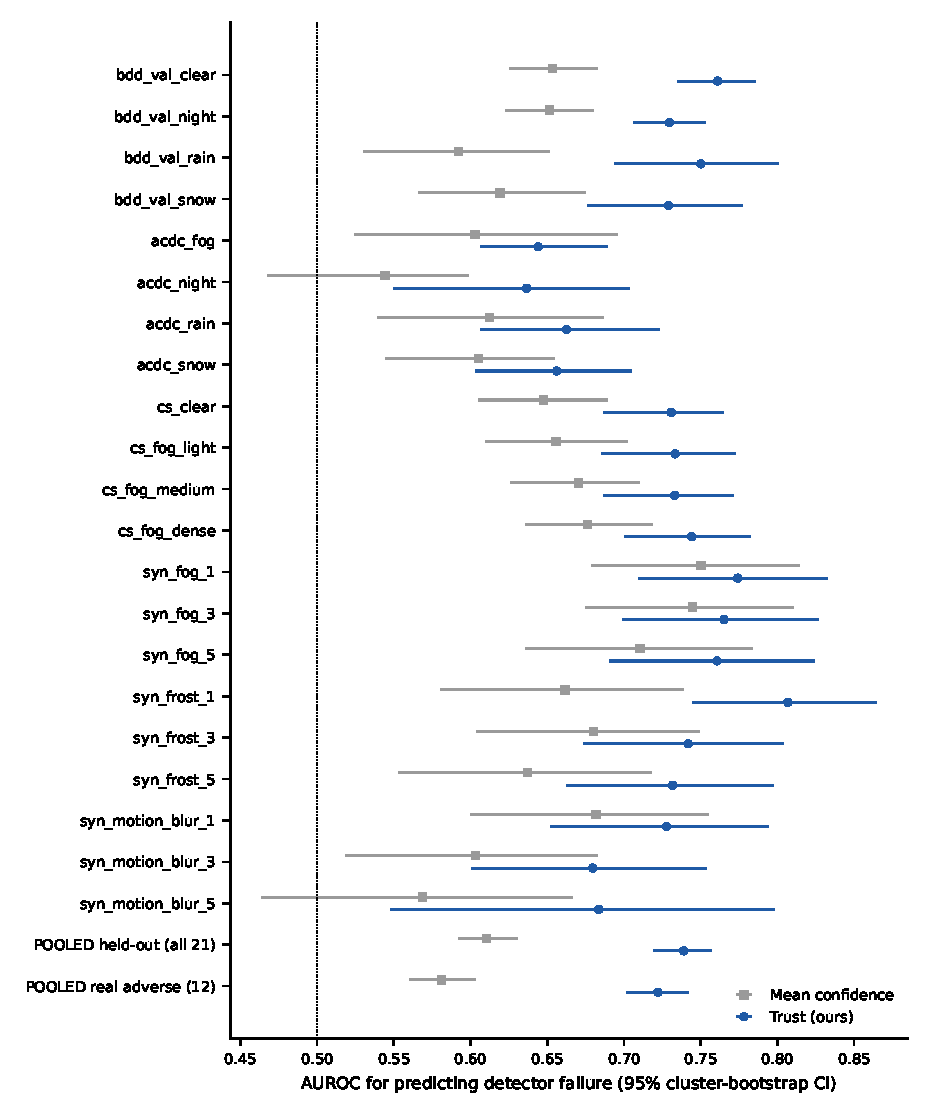
\includegraphics[width=0.85\linewidth]{figures/auroc_forest.pdf}
\caption{Failure-prediction AUROC per held-out stratum with 95\% cluster-bootstrap intervals}
\label{fig:forest}
\end{figure}

\subsection{Selective Prediction}

In operation, trust is meant to gate downstream decisions: a planner acts on frames whose trust is high and treats the remaining frames with caution. A useful trust score should therefore lower the failure rate among accepted frames as the accepted fraction (coverage) shrinks, and AURC and E-AURC (Eqs.~\ref{eq:aurc} and~\ref{eq:eaurc}) summarise this behaviour over all coverages (Table~\ref{tab:selective}, Fig.~\ref{fig:riskcov}). Over all held-out frames, E-AURC falls from 0.274 with mean confidence to 0.180 with trust, a 34\% reduction; over the real adverse strata it falls from 0.293 to 0.200 (32\%). Acting only on the most-trusted half of the frames reduces the failure rate from 55.6\% to 38.2\% pooled, from 36.8\% to 19.7\% on held-out clear frames and from 57.1\% to 40.9\% at night on BDD100K. Ranking by confidence lowers it only from 55.6\% to 47.6\%. A substantial gap to the oracle, which reaches 11.2\% at 50\% coverage, remains.

\begin{table}[t]
\caption{Selective prediction over pooled held-out frames: AURC and E-AURC (lower is better) and failure rate at several coverages}
\label{tab:selective}
\footnotesize
\setlength{\tabcolsep}{4pt}
\begin{tabular}{@{}llcccccc@{}}
\toprule
Pool & Score & AURC & E-AURC & @100\% & @80\% & @60\% & @50\% \\
\midrule
\multirow{3}{*}{All 21 held-out} & Confidence & 0.470 & 0.274 & 0.556 & 0.528 & 0.494 & 0.476 \\
& Trust & \textbf{0.375} & \textbf{0.180} & 0.556 & \textbf{0.483} & \textbf{0.415} & \textbf{0.382} \\
& Oracle & 0.196 & 0.000 & 0.556 & 0.445 & 0.260 & 0.112 \\
\midrule
\multirow{3}{*}{12 real adverse} & Confidence & 0.514 & 0.293 & 0.586 & 0.566 & 0.548 & 0.531 \\
& Trust & \textbf{0.420} & \textbf{0.200} & 0.586 & \textbf{0.521} & \textbf{0.456} & \textbf{0.425} \\
& Oracle & 0.221 & 0.000 & 0.586 & 0.482 & 0.309 & 0.171 \\
\bottomrule
\end{tabular}
\end{table}

\begin{figure}[t]
\centering
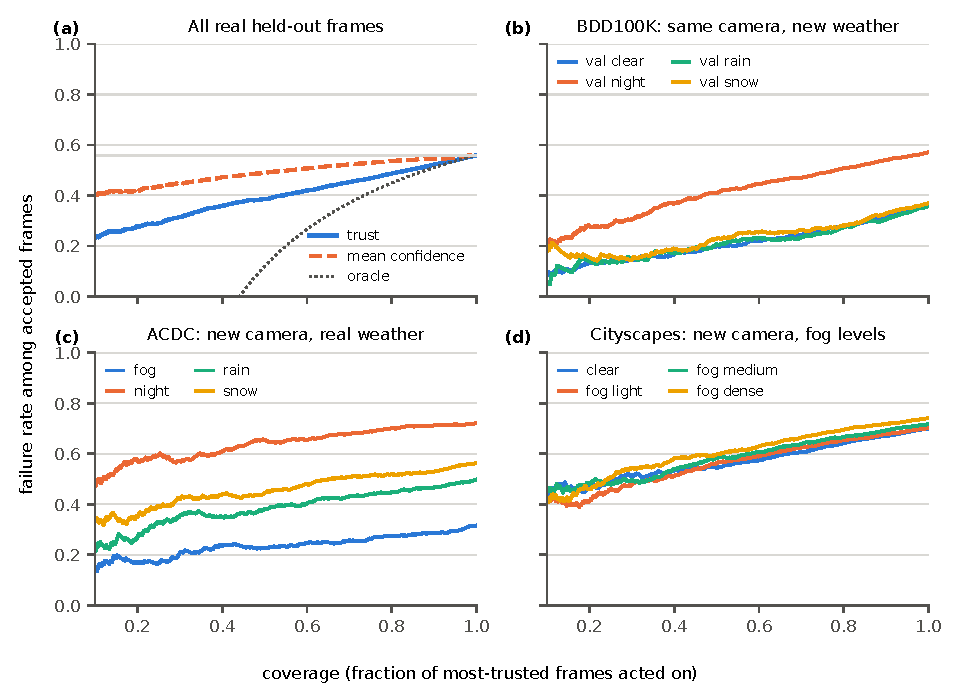
\includegraphics[width=\linewidth]{figures/risk_coverage_v2.pdf}
\caption{Risk--coverage curves on real held-out frames. (a) Trust, mean confidence and oracle, pooled; (b)--(d) trust per stratum for each kind of shift}
\label{fig:riskcov}
\end{figure}

\subsection{Calibration: Ranking Transfers, Probabilities Do Not}\label{sec:calib}

A score can order frames well and still give misleading probabilities. Calibration asks whether, among frames assigned a failure probability of, say, 0.7, about 70\% actually fail; it is measured by ECE (Eq.~\ref{eq:ece}) and the Brier score. Calibration is assessed on 20 of the 21 held-out strata: BDD100K validation clear is excluded because it is used below to fit the recalibration map. Pooled over these 20 strata, the raw failure probability $1-T$ has an ECE of 0.092 and a Brier score of 0.217. A common remedy is to recalibrate on held-out data, so isotonic regression~\cite{zadrozny2002isotonic} was fitted on the BDD100K validation clear frames and then frozen. On the shifted strata this made calibration \emph{worse}, raising the ECE to 0.148 and the Brier score to 0.229 (Fig.~\ref{fig:reliability}). The recalibration lowers predicted failure probabilities towards the 36.8\% clear-day base rate, while the adverse strata fail at rates of 32--82\%. Since the base rate of failure shifts with the conditions, a calibration map learned under one condition does not carry over to another. Trust should therefore be used as a ranking, or with condition-specific thresholds, rather than as a calibrated probability unless calibration data from the target condition is available. This agrees with the observation that post-hoc calibration does not survive dataset shift~\cite{ovadia2019trust}.

\begin{figure}[t]
\centering
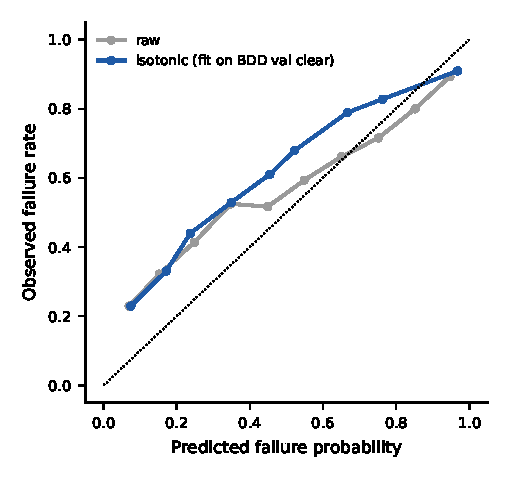
\includegraphics[width=0.5\linewidth]{figures/reliability.pdf}
\caption{Reliability of the predicted failure probability on shifted strata, before and after clear-day isotonic recalibration}
\label{fig:reliability}
\end{figure}

\subsection{Feature-Family Ablation}

To estimate how much each feature family contributes, the trust model was retrained with one family removed at a time. The pooled held-out AUROC is 0.739 for the full model, 0.690 without confidence statistics, 0.727 without image quality, 0.729 without the DINOv2 distance, 0.731 without flip-consistency and 0.741 without the weather probabilities. Confidence statistics are the most important family. Removing image quality, the DINOv2 distance or flip-consistency costs 0.008--0.012 each, which is less than the width of the pooled confidence interval ($\pm$0.02), so these individual contributions should be regarded as suggestive. The weather probabilities add nothing: the effect of weather is already visible in the other families, so the model does not need to be told which condition it is in. The most important single features are the number of detected persons, person flip-consistency, class entropy, overall flip-consistency and maximum confidence. A large number of detections is not the same as a large number of reliable detections, and only the combination of these signals captures the difference, which explains why the combined model outperforms any single confidence statistic.

\subsection{Danger Underestimation}\label{sec:res_danger}

If missed objects remove terms from Eq.~(\ref{eq:danger}), danger computed from detections should fall below danger computed from annotations, and the shortfall should grow with the severity of the conditions. The measured gap $\Delta$ confirms this expectation (Table~\ref{tab:danger}): detected danger underestimates true danger in every stratum, and every interval excludes zero. The gap is largest at night (0.091 on BDD100K and 0.104 on ACDC, with 36\% and 46\% of frames underestimated by more than 0.1), where missed pedestrians remove the highest-weight terms. On identical Cityscapes scenes it grows monotonically with fog density, from 0.019 to 0.042, and it grows with every synthetic corruption severity. $\Rest$ nevertheless preserves the ranking of scenes (Spearman correlation of 0.77--0.89 on the real strata), so the bias is systematic rather than random. Perturbing each class weight by $\pm$50\% leaves the frame ranking at a Spearman correlation of at least 0.954 and a high/medium/low tercile agreement of at least 0.875 over 2,000 frames, so the conclusions do not depend on the hand-set weights.

\begin{table}[t]
\caption{Danger gap $\Delta = \Rtrue - \Rest$ with 95\% cluster-bootstrap intervals, fraction of frames underestimated by more than 0.1 and Spearman correlation between $\Rest$ and $\Rtrue$}
\label{tab:danger}
\footnotesize
\setlength{\tabcolsep}{4pt}
\begin{tabular}{@{}lccccc@{}}
\toprule
Stratum & $\Rtrue$ & $\Rest$ & $\Delta$ [95\% CI] & $>0.1$ & $\rho_s$ \\
\midrule
BDD val clear & 0.618 & 0.597 & 0.021 [.017, .025] & 9.1\% & 0.83 \\
BDD val night & 0.718 & 0.627 & \textbf{0.091} [.084, .097] & \textbf{35.7\%} & 0.77 \\
BDD val rain & 0.741 & 0.710 & 0.031 [.024, .039] & 11.4\% & 0.85 \\
BDD val snow & 0.770 & 0.748 & 0.022 [.015, .030] & 9.2\% & 0.84 \\
ACDC fog & 0.668 & 0.654 & 0.014 [.004, .025] & 12.4\% & 0.89 \\
ACDC night & 0.614 & 0.511 & \textbf{0.104} [.083, .118] & \textbf{46.4\%} & 0.77 \\
ACDC rain & 0.561 & 0.531 & 0.030 [.026, .035] & 18.4\% & 0.87 \\
ACDC snow & 0.686 & 0.661 & 0.025 [.015, .036] & 15.2\% & 0.84 \\
Cityscapes clear & 0.641 & 0.622 & 0.019 [.016, .022] & 5.9\% & 0.89 \\
Cityscapes fog light & 0.791 & 0.767 & 0.024 [.020, .027] & 8.0\% & 0.89 \\
Cityscapes fog medium & 0.851 & 0.822 & 0.029 [.025, .033] & 9.8\% & 0.88 \\
Cityscapes fog dense & 0.911 & 0.868 & 0.042 [.037, .048] & 13.9\% & 0.87 \\
Synthetic fog 1 & 0.614 & 0.589 & 0.024 [.014, .036] & 8.0\% & 0.82 \\
Synthetic fog 3 & 0.614 & 0.584 & 0.030 [.018, .042] & 9.5\% & 0.81 \\
Synthetic fog 5 & 0.614 & 0.567 & 0.047 [.034, .061] & 14.5\% & 0.84 \\
Synthetic frost 1 & 0.614 & 0.569 & 0.045 [.034, .058] & 16.0\% & 0.81 \\
Synthetic frost 3 & 0.614 & 0.518 & 0.096 [.077, .115] & 30.0\% & 0.75 \\
Synthetic frost 5 & 0.614 & 0.496 & 0.117 [.098, .138] & 40.0\% & 0.71 \\
Synthetic blur 1 & 0.614 & 0.598 & 0.016 [.003, .029] & 9.0\% & 0.80 \\
Synthetic blur 3 & 0.614 & 0.568 & 0.046 [.028, .064] & 21.0\% & 0.67 \\
Synthetic blur 5 & 0.614 & 0.520 & 0.094 [.074, .114] & 39.0\% & 0.54 \\
\bottomrule
\end{tabular}
\end{table}

\subsection{Does the Decoupled Readout Isolate the Blind Spot?}

The motivation for keeping the two axes apart is the low-trust, low-apparent-danger quadrant: frames that a fused score would report as safe although perception is unreliable. To test whether this quadrant really concentrates underestimated danger, the held-out frames were cross-tabulated by both axes (Table~\ref{tab:quadrant}, Fig.~\ref{fig:quadrant}). Frames in this quadrant make up 7.8\% of the held-out frames; their mean danger gap is 0.192, and 65.7\% of them are underestimated by more than 0.1, compared with 13.5\% of frames outside it. They are also detector failures in 66.9\% of cases.

Two qualifications apply. First, most of the underestimation signal comes from the danger axis itself, since a low $\Rest$ leaves more room for underestimation. Within the low-apparent-danger frames, low trust raises the underestimation rate only from 57.7\% to 65.7\% and the mean gap from 0.153 to 0.192, although it raises the failure rate from 44.7\% to 66.9\%. Second, trust taken alone is a weak predictor of danger underestimation (pooled AUROC 0.55). It predicts whether detection failed, which includes false positives and missed cars, and not specifically whether hazard was missed. The quadrant is useful because it combines the two axes; neither axis alone identifies the blind spot. Training a trust model directly on the danger-gap target is a natural extension.

\begin{table}[t]
\caption{Held-out frames cross-tabulated by apparent danger ($\Rest < 0.4$) and trust ($T < 0.5$). ``Under'' = fraction with $\Delta > 0.1$}
\label{tab:quadrant}
\begin{tabular}{@{}llrcccc@{}}
\toprule
Apparent danger & Trust & Frames & Fail rate & Missed ped. & Mean $\Delta$ & Under \\
\midrule
High & High & 5,102 & 0.378 & 0.277 & 0.029 & 11.6\% \\
High & Low & 4,592 & 0.740 & 0.621 & 0.025 & 12.7\% \\
Low & High & 291 & 0.447 & 0.168 & 0.153 & 57.7\% \\
\textbf{Low} & \textbf{Low} & \textbf{839} & \textbf{0.669} & 0.229 & \textbf{0.192} & \textbf{65.7\%} \\
\bottomrule
\end{tabular}
\end{table}

\begin{figure*}[t]
\centering
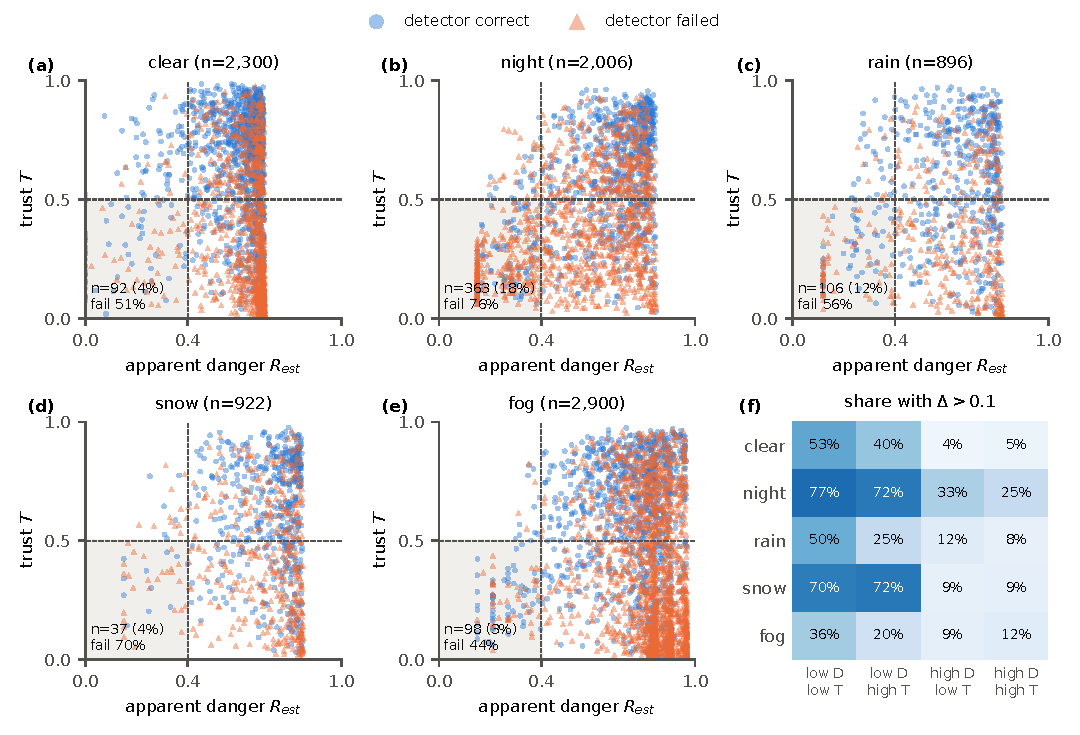
\includegraphics[width=\textwidth]{figures/quadrant_v2.pdf}
\caption{Trust against apparent danger on real held-out frames. (a)--(e) One panel per condition; the shaded corner is the low-trust, low-danger quadrant, annotated with its frame count and failure rate. (f) Share of frames whose danger is underestimated by more than 0.1, per condition and quadrant}
\label{fig:quadrant}
\end{figure*}

\subsection{Weather-Adaptive Enhancement}

Enhancement is worthwhile only if it recovers missed objects without making the detector more confident about wrong outputs. Both effects were measured by running the detector with enhancement on and off on identical frames (Table~\ref{tab:enh}). At night, enhancement adds 5.4--6.5 points of pedestrian recall, at a precision cost of 3.4 points on BDD100K. In dense fog it adds 4.2 points of recall and 2.8 points of mAP50, and the gains increase with fog density. In rain and snow the effect is within noise. The mean confidence of true positives changes by at most 0.012 in any stratum, so enhancement does not inflate confidence, and the trust layer, which reads its quality features from the raw frame, is not misled by it. The gains are modest, in line with the finding that restoration-oriented pre-processing helps recognition only partially~\cite{pei2018haze}.

\begin{table}[t]
\caption{Enhancement on minus off on identical frames (YOLO26m). Clear frames are untouched by design}
\label{tab:enh}
\footnotesize
\setlength{\tabcolsep}{4pt}
\begin{tabular}{@{}llcccc@{}}
\toprule
Stratum & Recipe & $\Delta$mAP50 & $\Delta$Ped.\ rec. & $\Delta$Prec. & $\Delta$TP conf. \\
\midrule
BDD val night & gamma, CLAHE, bilateral & $-$0.007 & \textbf{+0.065} & $-$0.034 & $-$0.002 \\
ACDC night & same & +0.011 & \textbf{+0.054} & +0.014 & +0.012 \\
BDD val rain & CLAHE & $-$0.004 & +0.007 & 0.000 & +0.002 \\
ACDC rain & CLAHE & $-$0.010 & +0.030 & +0.013 & $-$0.001 \\
BDD val snow & gamma, CLAHE & $-$0.001 & 0.000 & +0.003 & +0.002 \\
ACDC snow & gamma, CLAHE & 0.000 & +0.009 & +0.002 & +0.004 \\
ACDC fog & per fog level & +0.007 & +0.015 & $-$0.008 & +0.002 \\
Cityscapes fog light & CLAHE & +0.008 & +0.001 & $-$0.005 & +0.001 \\
Cityscapes fog medium & dehaze, CLAHE & +0.020 & +0.020 & $-$0.009 & +0.001 \\
Cityscapes fog dense & dehaze, CLAHE, denoise & +0.028 & \textbf{+0.042} & $-$0.021 & +0.001 \\
\bottomrule
\end{tabular}
\end{table}

\subsection{Weather Recognition}

The weather classifier drives both enhancement and one trust feature family, so its accuracy and its behaviour on unseen cameras matter for the rest of the pipeline (Table~\ref{tab:weather}). It reaches 99.72\% on the ACDC test split and 96.4\% on held-out BDD100K, where most remaining errors stem from noisy tags (wet roads tagged as rainy, snow on the ground tagged as snowy). On real Foggy Cityscapes frames from unseen cities, the fog level is exact in 97.85\% of frames and within one level in 99.9\%. Leave-one-camera-out accuracy is 93.9\%, which is the realistic figure for a new camera. Zero-shot CLIP~\cite{radford2021clip} is better only on DAWN's web imagery (82.7\% vs.\ 74.3\%), which resembles its pre-training data; on driving footage the trained model leads by 3--7 points and also provides the fog level.

\begin{table}[t]
\caption{Weather-condition accuracy on real test images}
\label{tab:weather}
\begin{tabular}{@{}lcccc@{}}
\toprule
Model & ACDC test & BDD100K test & DAWN (external) & Leave-one-camera-out \\
\midrule
CLIP zero-shot & 96.60\% & 89.03\% & \textbf{82.67\%} & -- \\
DINOv2 last-2 & 99.68\% & 95.85\% & 67.47\% & 93.91\% \\
ConvNeXt-T full & 99.08\% & 95.95\% & 72.73\% & 90.81\% \\
Ensemble & \textbf{99.72\%} & \textbf{96.36\%} & 74.29\% & -- \\
\bottomrule
\end{tabular}
\end{table}

\subsection{Runtime}

A trust signal is useful only if it is available while driving. At 1280$\times$720 with all components enabled (weather classification every 5 frames, mirrored pass every 2 frames, DINOv2 distance on), the pipeline sustains 20.6 frames per second, with p50/p95/p99 latencies of 47/71/81\,ms and a peak GPU memory of 439\,MB; process memory grows by 0.5\,MB over 300 frames. A fast preset, which skips the DINOv2 distance and runs the mirrored pass every 5 frames, reaches 34.8 frames per second (p95 54\,ms, 355\,MB). In the current implementation, however, the fast preset supplies zeros for the three distance features to a trust model trained with them. A zero distance signals maximal similarity to clear-day data, so trust in this mode is expected to be optimistic, and its accuracy was not measured. The ablation suggests that a model retrained without these features (AUROC 0.729) would lose little, and such a model should accompany the fast preset in deployment.

%% =====================================================================
\section{Discussion and Limitations}\label{sec:discussion}
%% =====================================================================

\textbf{Pooled gains are robust, gains on small strata are uncertain.} Cluster bootstrapping shows that the per-condition improvements on ACDC fog and rain and on several synthetic strata are not statistically significant. Benchmarks with few recordings per condition cannot support condition-level claims, and point estimates alone would have overstated consistency. Failure-prediction studies on adverse-weather data would benefit from reporting sequence-level intervals.

\textbf{Overfitting and training-set size.} The trust model attains an AUROC of 0.986 on its own training frames against 0.761 on held-out clear frames, which indicates substantial overfitting of the 400-tree model on 3,000 frames. Stronger regularisation, cross-validated hyperparameters and more clear-day training frames, which are cheap to obtain, are the most direct way to improve held-out performance.

\textbf{Overlap between classifier training and evaluation frames.} The ACDC and Cityscapes evaluation strata are drawn from the train and validation splits of those datasets, and the weather classifier was trained on their train splits. The weather-probability features are therefore partly in-sample on these frames. The ablation indicates that the pooled result does not depend on these features, since the trust model without them reaches the same pooled AUROC (0.741). The per-stratum values of the full model may nevertheless be slightly affected, and a re-evaluation restricted to the validation splits, which are disjoint from the classifier's training data, is the first check planned for future work.

\textbf{Baselines.} The comparison here is against mean detection confidence, the standard black-box baseline. Methods that access detector internals, such as MetaDetect~\cite{schubert2021metadetect} and the feature-based monitor of Rahman et al.~\cite{rahman2021online}, or that require multiple passes, such as ensembles~\cite{lakshminarayanan2017ensembles}, are complementary, and their comparison under the present protocol is left to future work.

\textbf{Danger formulation.} The danger score is hand-designed and image-based. Proximity is approximated from box size and position rather than metric depth, and no dataset provides near-miss labels against which danger could be validated externally. The claims of this paper therefore concern the \emph{difference} between the same formula evaluated on detections and on annotations, which does not depend on the formula's absolute validity, and the sensitivity analysis shows that this difference is robust to the weights.

\textbf{Single frames and a single detector.} The benchmarks consist of single images, so temporal consistency, potentially a strong failure signal, is replaced by flip-consistency. The trust model is specific to the chosen detector and must be retrained for another one, although its features require only black-box access.

\textbf{Calibration under shift.} Trust is a ranking that transfers, not a calibrated probability. Deployments that need probabilities should calibrate per condition, for example by letting the weather classifier select a calibration map fitted on a small annotated sample of each condition.

%% =====================================================================
\section{Conclusion}\label{sec:conclusion}
%% =====================================================================

This paper presented a perception readout that keeps two questions apart for every frame of monocular driving video: how far the detector can be trusted, and how dangerous the scene appears. A lightweight introspective model trained only on clear-day data predicts detector failure under unseen weather and cameras substantially better than detection confidence (pooled AUROC 0.739 vs.\ 0.610; E-AURC reduced by 34\%). The improvement is not significant on every small cross-camera condition, and the predicted probabilities do not remain calibrated under shift. Danger computed from detections is underestimated in every condition, most at night and increasingly with fog density, and the low-trust, low-apparent-danger quadrant isolates the frames in which this underestimation is concentrated. The pipeline runs in real time on a laptop GPU. Future work will train trust directly on the danger-gap target, exploit temporal consistency on video benchmarks, regularise and enlarge the training set, and compare against white-box failure predictors.

\backmatter

\bmhead{Acknowledgements}
The first author thanks Kulandai Josephine Julina Joseph for her supervision and guidance throughout this work. The authors thank the creators of BDD100K, ACDC, Cityscapes, Foggy Cityscapes and DAWN for making their datasets publicly available, and the authors of the works and open-source tools cited in this paper, on which this study builds.

\section*{Declarations}

\textbf{Author contributions} S. Arsalan: Conceptualization, Methodology, Software, Investigation, Formal analysis, Visualization, Writing -- original draft. K. J. J. Joseph: Supervision, Writing -- review \& editing.

\textbf{Funding} The authors received no specific funding for this work. %% TODO: confirm.

\textbf{Data availability} All datasets used (BDD100K, ACDC, Cityscapes, Foggy Cityscapes, DAWN) are publicly available from their providers. Per-frame trust and danger scores and all analysis scripts are available from the corresponding author and will be released upon acceptance.

\textbf{Conflicts of interest} The authors declare that they have no conflict of interest.

\bibliography{references}

\end{document}
